\section{Experiments and Results}
\begin{table}[t]
\centering
\caption{Prediction error (m) for 12 steps (4.8\,s). ETH is never seen in training or calibration.}
\label{tab:pred}
\setlength{\tabcolsep}{4pt}
\begin{tabular}{lcccc}
\toprule
& \multicolumn{2}{c}{Validation} & \multicolumn{2}{c}{ETH test}\\
\cmidrule(lr){2-3}\cmidrule(lr){4-5}
Predictor & ADE & FDE & ADE & FDE\\
\midrule
Constant velocity & 0.440 & 0.972 & 1.075 & 2.282\\
Kalman CV & 0.443 & 0.977 & 1.071 & 2.277\\
Social Force & 0.461 & 0.993 & 1.056 & 2.238\\
MLP & 0.431 & 0.938 & 1.030 & 2.091\\
LSTM & 0.440 & 0.958 & \textbf{1.003} & \textbf{2.045}\\
Temporal CNN & 0.430 & 0.936 & 1.021 & 2.058\\
Social-grid CNN & \textbf{0.429} & \textbf{0.934} & 1.044 & 2.155\\
\bottomrule
\end{tabular}
\end{table}

\begin{table}[t]
\centering
\caption{90\% uncertainty discs on ETH: empirical coverage and mean radius (m) at 1.6/3.2/4.8\,s.}
\label{tab:cov}
\setlength{\tabcolsep}{3.5pt}
\begin{tabular}{llcc}
\toprule
Pred. & Method & Coverage & Radius 1.6 / 3.2 / 4.8 s\\
\midrule
CV & split conformal & 57\% & 0.48 / 1.25 / 2.18\\
CV & speed-normalised conformal & 64\% & 0.65 / 1.74 / 3.03\\
CV & ACI & 90\% & 2.39 / 6.04 / 11.9\\
Kalman & filter covariance & 98\% & 1.84 / 4.85 / 8.69\\
LSTM & speed-normalised conformal & 65\% & 0.63 / 1.67 / 2.88\\
LSTM & ACI & 90\% & 1.67 / 3.74 / 6.86\\
GP & predictive $\sigma$ & 61\% & 0.49 / 1.28 / 2.23\\
\bottomrule
\end{tabular}
\end{table}

\begin{table*}[t]
\centering
\caption{Navigation in the reactive crowd, 120 paired episodes per row. Contacts per episode with 95\% bootstrap interval.
Univ = mean contacts in the two dense university scenes. Time = mean time to goal when reached. Pushed = people displaced by the robot (m).}
\label{tab:nav}
\setlength{\tabcolsep}{5pt}
\begin{tabular}{lcccccccc}
\toprule
Predictor & ETH ADE (m) & Success (\%) & Reached (\%) & Contacts / ep & At-fault / ep & Univ contacts & Time (s) & Pushed (m)\\
\midrule
\tabinput{generated/tab_nav.tex}
\bottomrule
\end{tabular}
\end{table*}

\begin{table}[t]
\centering
\caption{Conformal margins in R3 (ST-A* + MPC). Level = coverage target of the speed-normalised disc.}
\label{tab:margin}
\setlength{\tabcolsep}{3pt}
\begin{tabular}{llcccccc}
\toprule
Pred. & Level & Succ. & Reach. & Cont. & Univ succ. & Stop & Pushed\\
& & (\%) & (\%) & /ep & (\%) & (\%) & (m)\\
\midrule
\tabinput{generated/tab_margin.tex}
\bottomrule
\end{tabular}
\end{table}


\subsection{Prediction and calibration}
Table~\ref{tab:pred} confirms the known picture \cite{scholler2020}: the
three classical predictors are within 5\% of each other, and every network
beats them, by about 10\% in FDE on the unseen ETH scene. The social-grid
CNN, which sees the neighbours, is best on validation, while the LSTM
transfers best to ETH.

Table~\ref{tab:cov} shows that the conformal guarantee does not survive
the move to ETH. People there walk about twice as fast as in the
validation scenes (median 1.01 vs 0.51\,m/s), so 90\% discs calibrated on
validation cover only 57--65\% of ETH. Normalising by speed recovers 7
points. ACI restores 90\% coverage, but ETH errors are heavy-tailed and
the discs grow to several metres. Here the better predictor pays off: with
ACI the LSTM needs discs about 30\% smaller than CV for the same coverage.
Model-based uncertainty is either over-confident (GP, 61\%) or very
conservative (Kalman, 98\% with discs 3--4$\times$ larger).

\subsection{Navigation}
Table~\ref{tab:nav} and Fig.~\ref{fig:acc} give the main result. With 120
episodes a success rate has a standard error of about 4.5 points, so we
compare contacts, which are paired and more sensitive.

\emph{Using any prediction helps, and helps more the better the planner
can use it.} Constant-velocity prediction lowers contacts from 2.28 to
1.47 per episode with R1, from 1.23 to 0.87 with R2 ($-0.36$, 95\% CI
$[-0.61,-0.11]$, $p=0.011$) and from 1.47 to 0.67 with R3 ($-0.80$,
$[-1.10,-0.51]$, $p<0.001$). Without prediction, ST-A* is worse than
2-D A*: a space-time plan built on people standing still is confidently
wrong. With prediction it is the best planner.

\emph{The planner and controller matter more than the predictor.} With CV
prediction, replacing pure pursuit by DWA removes 0.60 contacts per episode
($[-0.93,-0.30]$, $p=0.010$), and replacing 2-D A* + DWA by ST-A* + MPC
removes another 0.20 ($[-0.38,-0.03]$, $p=0.017$). In the dense
university scenes contacts fall from 3.00 to 1.43 to 0.80 per episode and
success rises from 15\% to 20\% to 30\%. Pure pursuit is never at fault,
but it stops in people's way 13\% of the time and pushes them most
(0.42\,m); DWA and MPC almost never stop and disturb people about half as
much, at the cost of 0.4--0.5 at-fault contacts per episode.

\emph{Prediction accuracy does not translate into safety.} In R3, every
other predictor has slightly \emph{more} contacts than CV (0.75--0.78 vs
0.67), and no paired difference is significant ($+0.08$ to $+0.11$,
$p\ge0.23$). In R2 the predictors range from 0.77 to 0.93 contacts with
no link to accuracy: the LSTM, best on ETH, is last. Across the seven R3
predictors the rank correlation between ETH FDE and contacts is
$\rho=-0.71$ ($p=0.07$), i.e.\ if anything the less accurate predictors
are safer. Goal-reaching and time are also flat (LSTM reaches the goal
most often, 97\%, and the social-grid CNN is fastest, 22.8\,s). This
extends the finding of Poddar et al.\ \cite{poddar2023} from one deep
predictor to six predictors and three planners.

\emph{Replayed crowds overstate the risk.} The same R3 with CV has 0.92
contacts per episode when people are replayed and 0.67 when they react
($-0.25$, $[-0.37,-0.13]$, $p=0.002$), while at-fault contacts stay at
0.45--0.47: the extra contacts in replay are people walking into the
robot.

\begin{figure}[t]
\centering
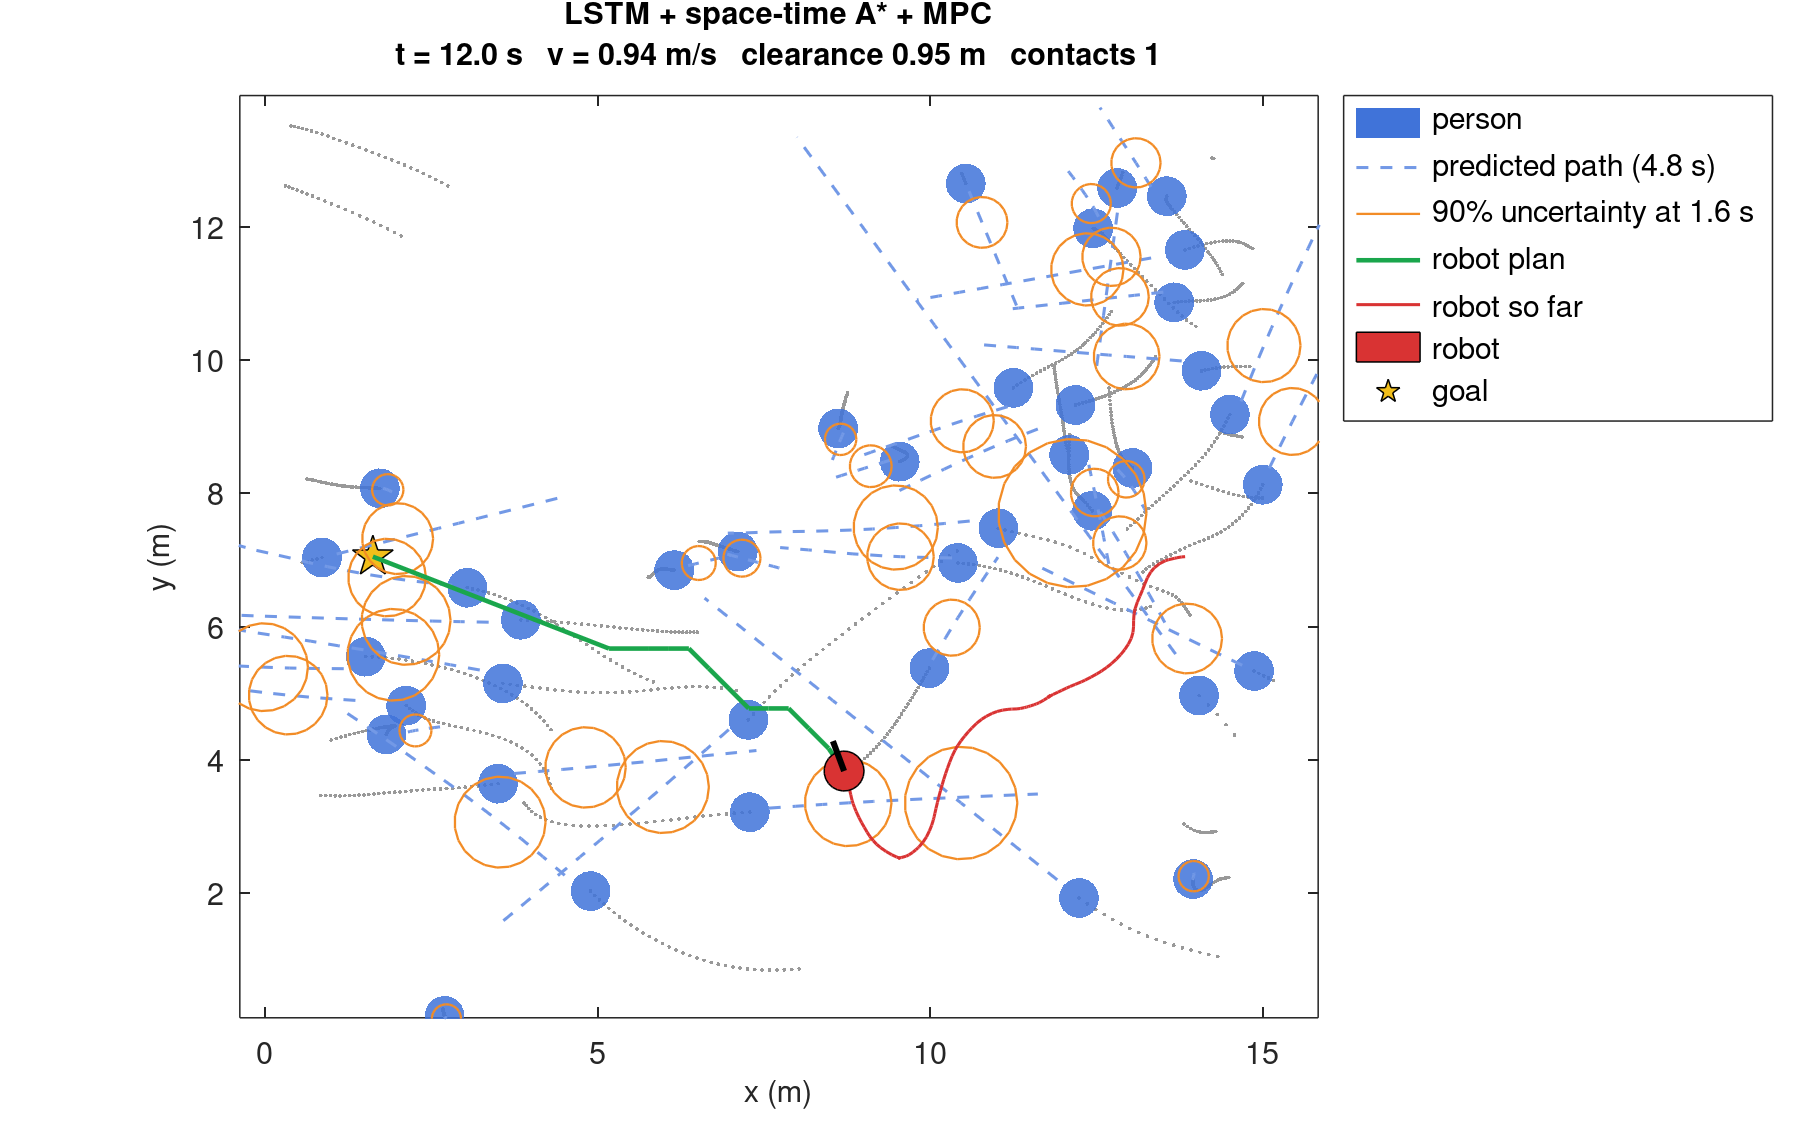
\includegraphics[width=\columnwidth]{fig_scene.png}
\caption{Students003 at $t=12$\,s with R3 and the LSTM predictor. Dashed:
4.8\,s LSTM predictions; orange: 90\% conformal discs at 1.6\,s (shown,
not used by this planner); green: space-time plan; red: path driven so
far; grey: recorded routes.}
\label{fig:scene}
\end{figure}

\begin{figure}[t]
\centering
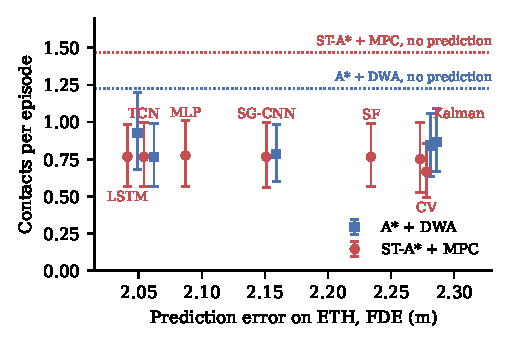
\includegraphics[width=\columnwidth]{fig_acc_safety.pdf}
\caption{Prediction error on ETH against contacts per episode (95\%
bootstrap intervals). Dotted lines: the same robot without prediction.}
\label{fig:acc}
\end{figure}

\begin{figure}[t]
\centering
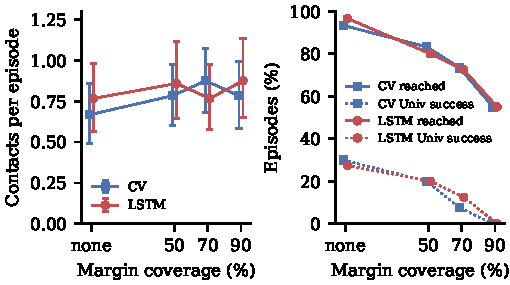
\includegraphics[width=\columnwidth]{fig_margin.pdf}
\caption{Conformal margins in R3. Left: contacts per episode (95\%
bootstrap intervals). Right: goal reached (solid) and success in the
university scenes (dotted).}
\label{fig:margin}
\end{figure}

\subsection{Uncertainty margins}
Table~\ref{tab:margin} and Fig.~\ref{fig:margin} add speed-normalised
conformal discs to every predicted person in R3. The margins make the robot
more cautious, as intended: people are displaced less (0.23 to
0.10\,m) and it stops more (1.5\% to 5.9\%). But they do not reduce
contacts. For CV, contacts go from 0.67 to 0.78, 0.88 and 0.78 at 50, 70
and 90\% coverage ($p=0.31$ and $0.40$ for 50\% and 90\%), and the LSTM
behaves the same way. Meanwhile the goal is reached in 93\%, 83\%, 73\%
and 55\% of episodes, success in the university scenes falls from 30\%
to 0\%, and travel time rises from 23.6 to 31.6\,s. This is the freezing
robot problem \cite{trautman2010}: with 90\% discs a fast walker's disc
is several metres wide at 3\,s, the space-time grid is blocked, and the
robot waits while people still reach it. With a replayed crowd and DWA
the same margins did cut contacts by about 20\% (1.06 to 0.86) in our
earlier runs; once people yield, the margins mostly cost progress.

\section{Discussion and Limitations}
\textbf{Why does accuracy not help?} Three effects combine. First, the
planner uses predictions only up to 3.2\,s ahead, and the gap between
predictors grows with the horizon; the 10\% FDE gain is at 4.8\,s.
Second, contacts in a reactive crowd are dominated by close-range
interaction, which the inflated hard obstacles and the controller's
clearance cost already handle. Third, the networks were trained on
recorded people who never met a robot. In our crowd people swerve
around the robot, and a model that smooths 8 observations (Kalman,
networks) reacts to a swerve later than CV, which uses only the last
step. Predictors trained or adapted in closed loop with the robot are the
natural next step.

\textbf{Where uncertainty helps.} Calibrated discs are only useful if the
planner can still move inside them. Under the ETH shift, guaranteed
coverage costs metres of room (Table~\ref{tab:cov}). A better predictor
shrinks the ACI discs by 30\%, which is the one place where accuracy paid
off in our study, and risk-weighted costs instead of hard discs
\cite{lindemann2023,dixit2023} are a promising way to use them.

\textbf{Limitations.} The crowd is a Social Force model driven by the
recordings, not real people; its reaction to a robot is a modelling
choice. All results are in simulation on six scenes, with one robot
model and 120 episodes per configuration, which resolves differences of
about 0.2 contacts per episode but not smaller ones. The networks are
small and deterministic; multi-modal generative predictors
\cite{gupta2018,salzmann2020} may behave differently.

\section{Conclusion}
We built a complete crowd-navigation stack in MATLAB with classical and
learned options at every layer, a leak-free ETH/UCY protocol and a
reactive crowd, and compared 23 configurations on the same 120 episodes.
Prediction itself matters: it halves contacts for a space-time planner.
But \emph{which} predictor matters little: six predictors that differ by
up to 10\% in displacement error give statistically identical navigation,
and the simplest is at least as safe. The choice of planner and controller
changes safety far more, with space-time A* and sampling MPC reducing
contacts by 54\% against A* with pure pursuit. Conformal margins are
calibrated only in distribution and, used as hard constraints, freeze the
robot in dense scenes. Navigation benchmarks should therefore report
closed-loop safety in reactive crowds, not displacement error alone.
Code, weights and results are public.
